\section{Algebra relazionale}

L'\textbf{algebra relazionale} è un linguaggio formale procedurale che
definisce un insieme di \textbf{operatori} applicabili a relazioni
(tabelle) e che producono come risultato \textbf{nuove relazioni}.
Essa costituisce il fondamento teorico dei linguaggi di interrogazione
dei database relazionali, come SQL.

Ogni operatore dell'algebra relazionale è \textbf{chiuso}, ovvero
restituisce sempre una relazione come risultato, permettendo la
composizione di più operatori in un'unica espressione.

La \textbf{segnatura} di un operatore descrive:
\begin{itemize}
	\item il numero di relazioni di input;
	\item l'eventuale presenza di parametri;
	\item il tipo del risultato prodotto.
\end{itemize}

Un \textbf{operatore unario} agisce su una singola relazione di input e
produce una relazione di output:

\[
Op_{\text{parametri}}(r_1) \;\rightarrow\; r_2
\]

dove:
\begin{itemize}
	\item $r_1$ è la relazione di input;
	\item $Op$ è l'operatore applicato;
	\item i \emph{parametri} specificano il comportamento dell'operatore;
	\item $r_2$ è la relazione risultante.
\end{itemize}

Un \textbf{operatore binario} agisce su due relazioni di input e produce
una nuova relazione:

\[
r_1 \; Op_{\text{parametri}} \; r_2 \;\rightarrow\; r_3
\]

dove:
\begin{itemize}
	\item $r_1$ e $r_2$ sono le relazioni di input;
	\item $Op$ è l'operatore binario;
	\item i \emph{parametri} definiscono le condizioni dell'operazione;
	\item $r_3$ è la relazione risultante.
\end{itemize}
\subsection{Classificazione degli operatori}

Gli operatori dell'algebra relazionale si classificano secondo due
criteri principali:

\subsubsection*{Classificazione funzionale}

\begin{itemize}
	\item Operatori insiemistici
	\item Operatori specifici
	\item Operatori di giunzione (join) tra relazioni
\end{itemize}

\subsubsection*{Classificazione in base alla derivabilità}

\begin{itemize}
	\item Operatori di base
	\item Operatori derivati
\end{itemize}
\subsection{Operatori insiemistici}

Poiché le relazioni sono insiemi di tuple, è naturale applicare ad esse
le operazioni dell'algebra degli insiemi.  
È tuttavia necessario ricordare che una relazione è un insieme di tuple
\textbf{omogenee}, cioè definite sullo stesso insieme di attributi
(stesso schema).

Di conseguenza, gli operatori insiemistici possono essere applicati
esclusivamente a relazioni che hanno \textbf{lo stesso schema}.

Dati due relazioni $r_1$ e $r_2$ definite sullo stesso schema $X$, si
definiscono i seguenti operatori:
\begin{figure}[H]
	\centering
	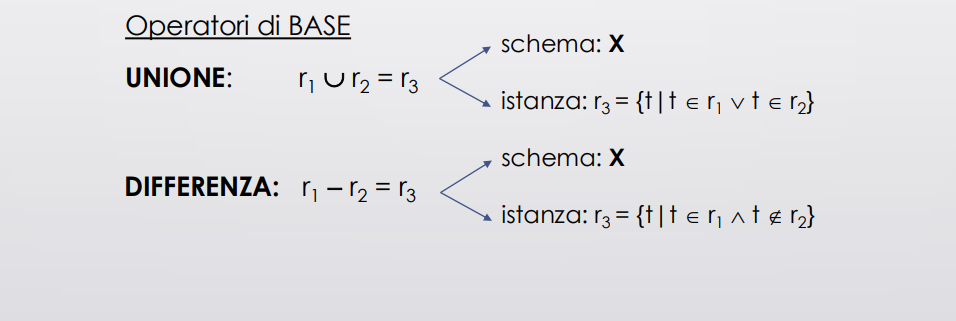
\includegraphics[width=1\linewidth]{image78}
	\caption{operazione di unione e differenza}
	\label{fig:image78}
\end{figure}
\begin{figure}[H]
	\centering
	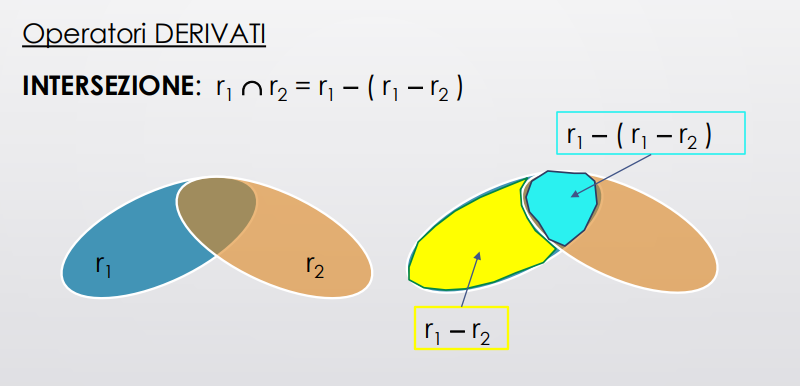
\includegraphics[width=1\linewidth]{image79}
	\caption{Intersezione}
	\label{fig:image79}
\end{figure}
\subsubsection{Cardinalità degli operatori insiemistici}

La \textbf{cardinalità} di una relazione indica il numero di tuple
contenute nella relazione risultante dall'applicazione di un operatore
dell'algebra relazionale.

\subsubsection*{Unione}

L'operatore di unione combina le tuple di due relazioni eliminando le
eventuali tuple duplicate.  
La cardinalità della relazione risultante dipende dal numero di tuple
comuni tra le due relazioni.

Il valore minimo si ottiene quando una relazione è interamente contenuta
nell'altra; in questo caso, la cardinalità dell'unione coincide con
quella della relazione più grande.  
Il valore massimo si ottiene quando le due relazioni non hanno tuple in
comune; in questo caso, la cardinalità dell'unione è pari alla somma
delle cardinalità delle due relazioni.

\[
\max(|r_1|, |r_2|) \;\le\; |r_1 \cup r_2| \;\le\; |r_1| + |r_2|
\]

\subsubsection*{Differenza}

L'operatore di differenza restituisce le tuple appartenenti alla prima
relazione che non sono presenti nella seconda relazione.  
La cardinalità della relazione risultante può variare da zero fino alla
cardinalità della prima relazione.

Il valore minimo si ottiene quando tutte le tuple della prima relazione
sono presenti anche nella seconda, producendo una relazione vuota.  
Il valore massimo si ottiene quando nessuna tupla della prima relazione è
presente nella seconda, per cui tutte le tuple della prima relazione
vengono mantenute.

\[
0 \;\le\; |r_1 - r_2| \;\le\; |r_1|
\]

\subsubsection*{Intersezione}

L'operatore di intersezione restituisce le tuple comuni a entrambe le
relazioni.  
La cardinalità della relazione risultante dipende quindi dal numero di
tuple condivise.

Il valore minimo si ottiene quando le due relazioni non hanno tuple in
comune, producendo una relazione vuota.  
Il valore massimo si ottiene quando la relazione più piccola è
interamente contenuta nella relazione più grande.

\[
0 \;\le\; |r_1 \cap r_2| \;\le\; \min(|r_1|, |r_2|)
\]
\subsection{Operatori specifici}
\subsubsection{Operatore di rinominaizone}
Dato una relazione $r$ definita sullo schema $X$, con
\[
X = \{A_1, \dots, A_n\},
\]
si definiscono i seguenti operatori.
L'operatore di \textbf{rinominazione} consente di modificare il nome degli
attributi di una relazione senza alterarne le tuple.  
Sia
\[
Y = \{B_1, \dots, B_n\}
\]
un insieme di attributi tale che $|Y| = |X|$.

La rinominazione è definita come:
\[
\rho_{A_1 \rightarrow B_1, \dots, A_n \rightarrow B_n}(r) = r_2
\]

dove:
\begin{itemize}
	\item lo schema della relazione risultante è $Y$;
	\item l'istanza $r_2$ contiene le stesse tuple di $r$;
	\item per ogni tupla $t \in r$ e per ogni $i \in \{1, \dots, n\}$,
	vale $t[B_i] = t[A_i]$.
\end{itemize}
\subsubsection*{Esempio}

Schema relazionale:
\begin{itemize}
	\item \texttt{CAPOLUOGO\_PROV(Nome, Popolazione, CAP)}
	\item \texttt{COMUNI\_MINORI(Nome, Abitanti, CAP)}
\end{itemize}

Per produrre la lista di tutti i comuni è necessario rendere compatibili
gli schemi delle due relazioni.  
Si applica quindi l'operatore di rinominazione per uniformare il nome
degli attributi:

\[
\rho_{\text{Popolazione} \rightarrow \text{Abitanti}}
(\text{CAPOLUOGO\_PROV}) \;\cup\; \text{COMUNI\_MINORI}
\]
Dato una relazione $r$ definita sullo schema $X$, con
\[
X = \{A_1, \dots, A_n\},
\]
si definiscono i seguenti operatori.
\subsubsection{Operatore di Selezione}
L'operatore di \textbf{selezione} consente di estrarre da una relazione le tuple
che soddisfano una determinata condizione.

La selezione è definita come:
\[
\sigma_F(r_1) = r_2
\]

dove:
\begin{itemize}
	\item lo schema della relazione risultante è lo stesso di $r_1$;
	\item l'istanza risultante è
	\[
	r_2 = \{\, t \mid t \in r_1 \land F(t) \,\};
	\]
	\item $F(t)$ indica che la tupla $t$ rende vera la formula $F$.
\end{itemize}

La formula $F(t)$ è una formula proposizionale ottenuta combinando,
mediante i connettivi logici $\land$, $\lor$ e $\neg$, condizioni
atomiche del tipo:
\[
A \; \theta \; B \quad \text{oppure} \quad A \; \theta \; c
\]

dove:
\begin{itemize}
	\item $A$ e $B$ sono attributi della relazione;
	\item $\theta \in \{=, \neq, >, \ge, <, \le\}$;
	\item $c$ è una costante appartenente al dominio di $A$ o compatibile
	con esso.
\end{itemize}

Una formula del tipo $A \; \theta \; B$ è vera sulla tupla $t$ se
$t[A] \; \theta \; t[B]$, mentre una formula del tipo
$A \; \theta \; c$ è vera se $t[A] \; \theta \; c$.

Le formule composte assumono valori booleani determinati dalle tavole di
verità dei connettivi logici utilizzati.
\subsubsection*{Esempio}

Schema relazionale:
\begin{itemize}
	\item \texttt{TRENO(Numero, PartOra, PartMin, Cat, Dest, ArrOra, ArrMin)}
	\item \texttt{FERMATA(NumTreno, Stazione, Ora, Min)}
\end{itemize}

Si richiede di produrre la lista di tutti i treni non regionali che
partono alle ore 12:00 o dopo le 12:00 e prima delle 16:00.

L'espressione in algebra relazionale è:
\[
\sigma_{\text{PartOra} \ge 12 \;\land\; \text{PartOra} < 16 \;\land\;
	\text{Cat} \neq \text{'REGIONALE'}}(\text{TRENO})
\]
\subsubsection{Proiezione}

L'operatore di proiezione consente di ridurre una relazione eliminando
alcuni attributi, mantenendo solo quelli di interesse.  
La riduzione avviene in senso verticale.

Sia $Y = \{A_1, \dots, A_m\} \subseteq X$ un sottoinsieme degli attributi
dello schema $X$ della relazione $r_1$.

La proiezione è definita come:
\[
\pi_Y(r_1) = r_2
\]

dove:
\begin{itemize}
	\item lo schema della relazione risultante è $Y$;
	\item l'istanza risultante è
	\[
	r_2 = \{\, t \mid \exists t' \in r_1 : t'[Y] = t \,\};
	\]
	\item $t'[Y]$ indica la tupla ottenuta da $t'$ considerando solo gli
	attributi appartenenti a $Y$;
	\item eventuali tuple duplicate vengono eliminate.
\end{itemize}
\subsubsection*{Esempio}

Schema relazionale:
\begin{itemize}
	\item \texttt{TRENO(Numero, PartOra, PartMin, Cat, Dest, ArrOra, ArrMin)}
	\item \texttt{FERMATA(NumTreno, Stazione, Ora, Min)}
\end{itemize}

Si richiede di estrarre il \textbf{numero} e l'\textbf{ora di partenza}
dei treni \textit{Freccia Rossa} (categoria = \texttt{'FR'}) con
destinazione \textit{Milano Centrale}.

L'espressione in algebra relazionale è:
\[
\pi_{\text{Numero}, \text{PartOra}}
\big(
\sigma_{\text{Dest} = \text{'Milano Centrale'} \;\land\;
	\text{Cat} = \text{'FR'}}
(\text{TRENO})
\big)
\]
\subsubsection{Cardinalità degli operatori specifici}

La cardinalità indica il numero di tuple contenute nella relazione risultato di un'operazione di algebra relazionale.

\paragraph{Selezione:}
L'operatore di selezione $\sigma$ filtra le tuple di una relazione in base a una condizione logica, senza modificare gli attributi.

La cardinalità della relazione risultante soddisfa la seguente relazione:
\[
0 \le |\sigma_F(r_1)| \le |r_1|
\]

Questo significa che:
\begin{itemize}
	\item la selezione può restituire nessuna tupla;
	\item può restituire tutte le tuple della relazione originale;
	\item non può mai aumentare il numero di tuple.
\end{itemize}

\paragraph{Proiezione}
L'operatore di proiezione $\Pi$ seleziona un sottoinsieme di attributi della relazione ed elimina eventuali tuple duplicate.

La cardinalità della relazione risultante è compresa tra:
\[
\min(|r_1|, 1) \le |\Pi_Y(r_1)| \le |r_1|
\]

In particolare:
\begin{itemize}
	\item la proiezione può ridurre il numero di tuple a causa dell'eliminazione dei duplicati;
	\item nel caso migliore, la cardinalità rimane invariata.
\end{itemize}

Se l'insieme di attributi $Y$ è una superchiave per la relazione $r_1$, allora non si generano duplicati e vale:
\[
|\Pi_Y(r_1)| = |r_1|
\]

\subsubsection{Operatori di giunzione (JOIN)}

Dati due relazioni $r_1$ e $r_2$ con schema rispettivamente $X_1$ e $X_2$, 
gli operatori di \textit{join} generano tuple nella relazione risultato 
a partire da coppie di tuple $(t_1, t_2) \in r_1 \times r_2$ che soddisfano 
una determinata condizione, detta \textit{predicato di join}.

\subsubsection{JOIN naturale}
Il join naturale è un operatore di base in cui il predicato di join è 
definito automaticamente sugli attributi comuni alle due relazioni.
Tale operatore è quindi dipendente dallo schema.

Lo schema della relazione risultante è:
\[
\text{schema}(r_3) = X_1 \cup X_2
\]

dove gli attributi comuni compaiono una sola volta.

L'istanza della relazione risultato è definita come:
\[
r_3 = \{\, t \mid \exists t_1 \in r_1,\ \exists t_2 \in r_2 :
t[X_1] = t_1 \land t[X_2] = t_2 \,\}
\]

Il predicato di join è una condizione di uguaglianza sugli attributi comuni
alle due relazioni.
\subsubsection*{Esempio}

Si consideri il seguente schema relazionale:

\[
\text{DOCENTE}(\underline{CFDocente}, Nome, Cognome)
\]
\[
\text{CORSO}(Nome, \underline{CFDocente})
\]

Si richiede di produrre l’insieme dei corsi riportando il nome del corso
e il cognome del docente che lo tiene.

Poiché le informazioni richieste sono distribuite su due relazioni
diverse, è necessario applicare un operatore di join.
Il collegamento tra le relazioni avviene tramite l’attributo comune
\texttt{CFDocente}.

Dal momento che l’attributo \texttt{Nome} della relazione \texttt{CORSO}
deve essere rinominato in \texttt{NomeCorso}, si applica preliminarmente
l’operatore di rinomina.

L’espressione di algebra relazionale è la seguente:

\[
\Pi_{NomeCorso,\, Cognome}
\Big(
\rho_{Nome \rightarrow NomeCorso}(\text{CORSO})
\;\bowtie\;
\text{DOCENTE}
\Big)
\]

L’operatore di join naturale combina le tuple delle due relazioni
sulla base dell’uguaglianza dell’attributo comune \texttt{CFDocente}.
Successivamente, la proiezione consente di ottenere esclusivamente
gli attributi richiesti nel risultato finale.

\begin{figure}[H]
	\centering
	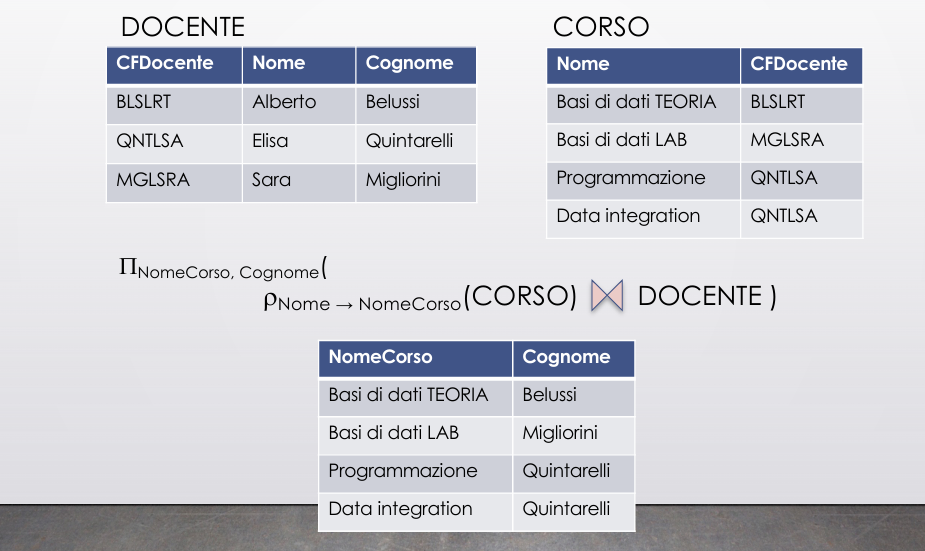
\includegraphics[width=1\linewidth]{image80}
	\caption{Esempio più visivo del JOIN naturale}
	\label{fig:image80}
\end{figure}
\subsubsection*{Proprietà del JOIN naturale}

Il join naturale tra due relazioni $r_1$ e $r_2$ si dice \emph{completo}
se tutte le tuple delle due relazioni contribuiscono a generare
almeno una tupla nella relazione risultato.

Formalmente, il join naturale è completo se valgono entrambe le seguenti
condizioni:

\[
\forall t_1 \in r_1:\ \exists t \in r_1 \bowtie r_2 \ \text{tale che} \ t[X_1] = t_1
\]

\[
\forall t_2 \in r_2:\ \exists t \in r_1 \bowtie r_2 \ \text{tale che} \ t[X_2] = t_2
\]

Queste condizioni garantiscono che ogni tupla di $r_1$ e di $r_2$
compaia almeno una volta nel risultato del join.

Se il join naturale non è completo, le tuple che non contribuiscono
alla generazione di alcuna tupla nel risultato si dicono
\textbf{dangling tuples}.
Il join naturale gode di alcune proprietà algebriche analoghe a quelle
degli operatori classici dell'algebra.

\paragraph{Commutatività:}
Il join naturale è commutativo:
\[
r_1 \bowtie r_2 = r_2 \bowtie r_1
\]

\paragraph{Associatività:}
Il join naturale è associativo:
\[
r_1 \bowtie (r_2 \bowtie r_3) = (r_1 \bowtie r_2) \bowtie r_3
\]

\paragraph{Relazioni con lo stesso schema:}
Se le relazioni $r_1$ e $r_2$ hanno lo stesso schema, allora il join
naturale coincide con l'intersezione:
\[
r_1 \bowtie r_2 = r_1 \cap r_2
\]

\paragraph{Assenza di attributi comuni:}
Se le relazioni $r_1$ e $r_2$ non hanno attributi in comune, allora il
join naturale coincide con il prodotto cartesiano:
\[
r_1 \bowtie r_2 = r_1 \times r_2
\]
\subsubsection{Cardinalità del JOIN naturale}
In generale, la cardinalità del join naturale tra due relazioni $r_1$ e $r_2$
è compresa tra zero e il prodotto delle cardinalità delle due relazioni:
\[
0 \le |r_1 \bowtie r_2| \le |r_1| \cdot |r_2|
\]

Se il join naturale è completo, allora ogni tupla di entrambe le relazioni
contribuisce a generare almeno una tupla nel risultato, e vale:
\[
\max(|r_1|, |r_2|) \le |r_1 \bowtie r_2| \le |r_1| \cdot |r_2|
\]

Se l’insieme degli attributi comuni $X_1 \cap X_2$ è una superchiave per
la relazione $r_2$, allora a ogni tupla di $r_1$ può corrispondere al più
una tupla di $r_2$, e quindi:
\[
0 \le |r_1 \bowtie r_2| \le |r_1|
\]

Se $X_1 \cap X_2$ è una superchiave per $r_2$ ed esiste un vincolo di
integrità referenziale tra $X_1 \cap X_2$ (o una sua parte) di $r_1$ e $r_2$,
allora ogni tupla di $r_1$ trova corrispondenza in $r_2$ e vale:
\[
|r_1 \bowtie r_2| = |r_1|
\]
\newpage
\subsubsection{THETA JOIN}
Date due relazioni \( r_1 \) e \( r_2 \) di schema \( X_1 \) e \( X_2 \) rispettivamente,
si introduce, oltre al \textit{join naturale}, il seguente operatore.
\textbf{Theta Join}: il predicato di join viene indicato esplicitamente
ed è indipendente dallo schema delle relazioni.

\subsubsection*{Precondizione}
Gli schemi delle relazioni devono essere disgiunti:
\[
X_1 \cap X_2 = \emptyset
\]


\subsubsection*{Definizione}
Il theta join è definito come una selezione applicata al prodotto cartesiano:
\[
r_1 \bowtie_\theta r_2 = \sigma_\theta ( r_1 \times r_2 )
\]

dove:
\begin{itemize}
	\item \( \times \) è il prodotto cartesiano
	\item \( \sigma_\theta \) è l’operatore di selezione
	\item \( \theta \) è un predicato conforme alla sintassi della selezione
\end{itemize}

Il predicato \( \theta \) può contenere confronti tra attributi delle due relazioni
utilizzando operatori di confronto come \( =, \neq, <, >, \leq, \geq \).

\begin{figure}[H]
	\centering
	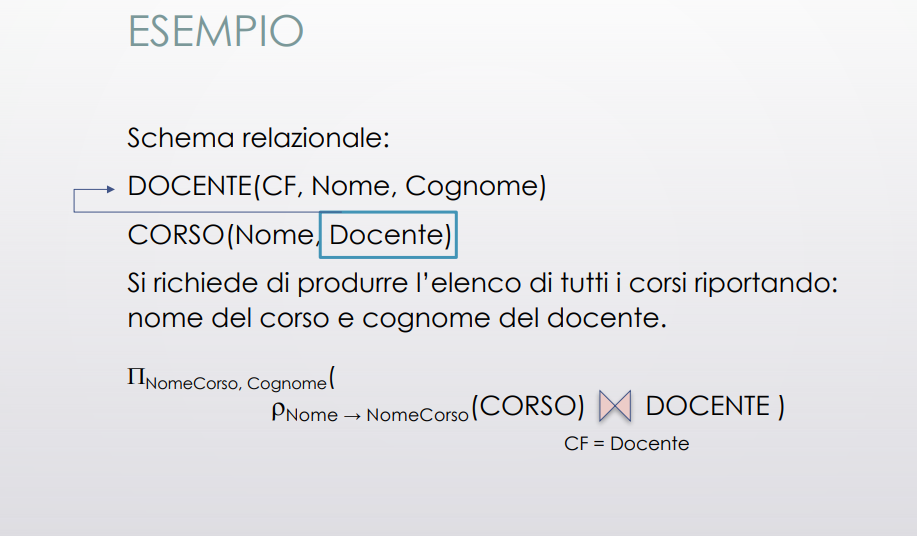
\includegraphics[width=1\linewidth]{image81}
	\caption{Esempio dell'uso del Theta Join}
	\label{fig:image81}
\end{figure}
\subsection*{Proprietà del Theta Join}

Il \textbf{theta join} si dice \textbf{equi-join} se la condizione
\( \theta \) è una congiunzione di uguaglianze:

\[
r_1 \;\bowtie_{\;A_1 = B_1 \;\wedge\; \dots \;\wedge\; A_n = B_n}\; r_2
\]

\bigskip

\noindent
\textbf{N.B.:} \textbf{ATTENZIONE} non esiste un operatore misto che applica
la logica del \emph{join naturale} per gli attributi comuni e aggiunge
ulteriori condizioni specificate esplicitamente tramite il predicato
\( \theta \).\\
\textbf{Teorema}

Date due relazioni \( r_1 \) e \( r_2 \) di schema \( X_1 \) e \( X_2 \) con
\[
X_1 \cap X_2 = \{ C_1, \dots, C_m \} \quad \text{con } m > 0,
\]
vale la seguente equivalenza:

\[
r_1 \bowtie r_2
=
\Pi_{X_1 \cup X_2}
\left(
r_1
\;\bowtie_{\;C_1 = C'_1 \;\wedge\; \dots \;\wedge\; C_m = C'_m}\;
\rho_{C_1, \dots, C_m \rightarrow C'_1, \dots, C'_m}(r_2)
\right)
\]


\paragraph{Ridenominazione}
Data la relazione \( r_1 \) di schema
\[
X_1 = \{ A_1, \dots, A_n \},
\]
per cambiare nome a tutti gli attributi si può scrivere:

\[
\rho_{A_1, \dots, A_n \rightarrow A'_1, \dots, A'_n}(r_1)
\]

oppure, in forma breve:

\[
\rho_{X \rightarrow X'}(r_1)
\]

\bigskip

\noindent
\textbf{N.B.:} \textbf{non sono ammesse} notazioni simili alla \emph{dot notation}
per indicare l’attributo di una tabella.

\noindent
La notazione \( T.A \) (per indicare l’attributo \( A \) della tabella \( T \))
\textbf{NON è una notazione ammessa dall’algebra relazionale}.
\subsection{Algebra con valori nulli}
È opportuno estendere l’algebra relazionale affinché possa operare anche su relazioni che contengono valori nulli.
In particolare, è necessario definire in modo esplicito il comportamento delle operazioni che coinvolgono il
confronto tra attributi, poiché la presenza di valori nulli introduce ambiguità semantiche.

Le operazioni che richiedono una gestione specifica dei valori nulli sono:
\begin{itemize}
	\item \textbf{Selezione}
	\item \textbf{Join naturale}
\end{itemize}

Le altre operazioni dell’algebra relazionale (proiezione, unione, differenza e prodotto cartesiano) 
si limitano a propagare i valori nulli eventualmente presenti nelle tuple di input, senza introdurre
nuove problematiche semantiche.

\medskip

\noindent
\textbf{Motivazione:}
La selezione e il join naturale si basano su confronti tra valori di attributi.
In presenza di valori nulli, tali confronti non possono essere valutati secondo la logica booleana classica,
ma richiedono una logica a tre valori (\textit{vero}, \textit{falso}, \textit{sconosciuto}).
Per questo motivo, è necessario estendere formalmente l’algebra relazionale per garantire
un comportamento coerente e ben definito di queste operazioni.
\subsubsection{Selezione}

Le condizioni di selezione in presenza di valori nulli assumono i seguenti valori di verità:

\begin{itemize}
	\item Sia $A \,\theta\, B$ una condizione atomica applicata a una tupla $t$.
	Se $t[A] = \text{NULL}$ oppure $t[B] = \text{NULL}$, allora l’espressione
	$t[A] \,\theta\, t[B]$ è valutata come \textbf{FALSO}.
	
	\item Sia $A \,\theta\, c$ una condizione atomica applicata a una tupla $t$, dove $c$ è una costante.
	Se $t[A] = \text{NULL}$, allora l’espressione
	$t[A] \,\theta\, c$ è valutata come \textbf{FALSO}.
	
	\item Sono introdotte le seguenti condizioni atomiche aggiuntive:
	\[
	A \ \text{IS NULL} \qquad \text{e} \qquad A \ \text{IS NOT NULL}.
	\]
	L’espressione $A \ \text{IS NULL}$, valutata sulla tupla $t$, è \textbf{VERO} se $t[A] = \text{NULL}$,
	altrimenti è \textbf{FALSO}.  
	Viceversa, l’espressione $A \ \text{IS NOT NULL}$ è \textbf{VERO} se $t[A] \neq \text{NULL}$,
	altrimenti è \textbf{FALSO}.
\end{itemize}
\subsubsection{Join naturale}

Nel join naturale, la condizione di uguaglianza sugli attributi comuni alle due relazioni
è valutata come \textbf{FALSA} sulle tuple $t_1$ e $t_2$ se almeno uno degli attributi comuni
di $t_1$ oppure di $t_2$ assume valore \texttt{NULL}.

\medskip

Si osservi, in particolare, che il confronto
\[
\texttt{NULL} = \texttt{NULL}
\]
è sempre valutato come \textbf{FALSO}.
\subsection{Ottimizzazione di espressioni DML}
Ogni espressione DML (generalmente specificata tramite un linguaggio dichiarativo)
ricevuta dal DBMS è sottoposta a un processo di elaborazione e ottimizzazione
prima della sua esecuzione.

\begin{figure}[H]
	\centering
	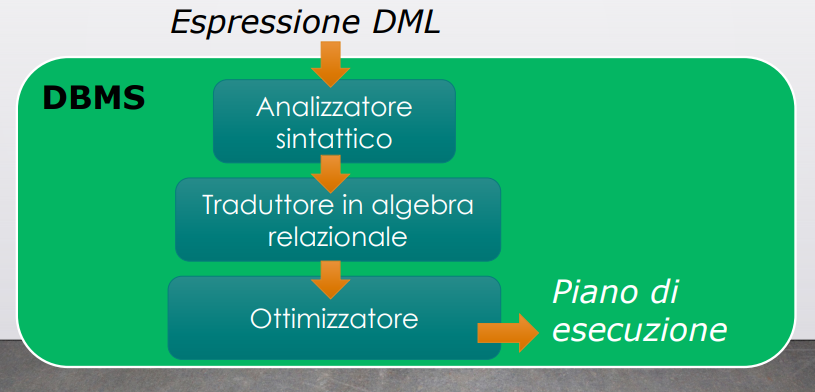
\includegraphics[width=\linewidth]{image82}
	\caption{Ottimizzazione di espressioni DML}
	\label{fig:image82}
\end{figure}

L’ottimizzatore genera un’espressione equivalente a quella di input, ma caratterizzata
da un costo inferiore.
Il costo viene stimato principalmente in termini di dimensione dei risultati intermedi,
numero di accessi ai dati e operazioni eseguite.

\medskip

Per ridurre il costo complessivo dell’esecuzione, l’ottimizzatore applica
trasformazioni di equivalenza sull’espressione di input,
con l’obiettivo di minimizzare la dimensione dei risultati intermedi e migliorare
l’efficienza dell’elaborazione.
\subsection{Equivalenza tra espressioni algebriche}

\subsubsection{Equivalenza dipendente dallo schema}

Dato uno schema $R$, due espressioni algebriche $E_1$ ed $E_2$ si dicono
\emph{equivalenti rispetto allo schema $R$}, e si scrive:
\[
E_1 \equiv_R E_2
\]
se vale che
\[
E_1(r) = E_2(r) \quad \text{per ogni istanza } r \text{ dello schema } R.
\]

\medskip

\noindent
\textbf{Esempio:}
\[
\Pi_{AB}(R_1) \;\bowtie\; \Pi_{AC}(R_2)
\;\equiv_R\;
\Pi_{ABC}(R_1 \;\bowtie\; R_2)
\]

\subsubsection{Equivalenza assoluta}

L’equivalenza assoluta è indipendente dallo schema.
Due espressioni $E_1$ ed $E_2$ si dicono \emph{assolutamente equivalenti}, e si scrive:
\[
E_1 \equiv E_2
\]
se vale che
\[
E_1 \equiv_R E_2 \quad \text{per ogni schema } R \text{ compatibile con } E_1 \text{ ed } E_2.
\]

\medskip

\noindent
\textbf{Esempio:}
\[
\Pi_{AB}(\sigma_{A>0}(R)) \;\equiv\; \sigma_{A>0}(\Pi_{AB}(R))
\]

% --------------------------------------------------

\subsection{Trasformazioni di equivalenza}

Sia $E$ un’espressione di schema $X$. Si definiscono le seguenti trasformazioni
di equivalenza.

\subsubsection*{Atomizzazione delle selezioni}

\[
\sigma_{F_1 \land F_2}(E) \;\equiv\; \sigma_{F_1}(\sigma_{F_2}(E))
\]

Questa trasformazione è propedeutica ad altre trasformazioni.
Da sola non produce un’ottimizzazione se non è seguita da ulteriori riscritture.

\subsubsection{Idempotenza delle proiezioni}

\[
\Pi_Y(E) \;\equiv\; \Pi_Y(\Pi_Z(E)) \qquad \text{con } Z \subseteq X
\]

Anche questa trasformazione è propedeutica e non comporta
un’ottimizzazione se applicata isolatamente.

% --------------------------------------------------

\subsection{Trasformazioni di equivalenza con il join}

Siano $E_1$ ed $E_2$ espressioni di schema rispettivamente $X_1$ e $X_2$.

\subsubsection*{Anticipazione delle selezioni rispetto al join}

\[
\sigma_F(E_1 \bowtie E_2) \;\equiv\; E_1 \bowtie \sigma_F(E_2)
\]

La trasformazione è applicabile solo se la condizione $F$ fa riferimento
esclusivamente ad attributi di $E_2$.

\subsubsection*{Anticipazione della proiezione rispetto al join}

\[
\Pi_{X_1 \cup Y}(E_1 \bowtie E_2) \;\equiv_R\; E_1 \bowtie \Pi_Y(E_2)
\]


La trasformazione è applicabile solo se:
\[
Y \subseteq X_2
\quad \mbox{e} \quad
(X_2 - Y) \cap X_1 = \emptyset
\]

% --------------------------------------------------

\subsection{Combinazione di anticipazione e idempotenza}

Combinando l’anticipazione della proiezione con l’idempotenza delle proiezioni
si ottengono le seguenti equivalenze:

\[
\Pi_Y(E_1 \bowtie_F E_2)
\;\equiv\;
\Pi_Y\bigl(\Pi_{Y_1}(E_1) \bowtie_F \Pi_{Y_2}(E_2)\bigr)
\]


\[
\Pi_Y(E_1 \bowtie E_2)
\;\equiv\;
\Pi_Y\bigl(\Pi_{Y_1}(E_1) \bowtie \Pi_{Y_2}(E_2)\bigr)
\]

dove:
\begin{itemize}
	\item $Y_1 = (X_1 \cap Y) \cup J_1$
	\item $Y_2 = (X_2 \cap Y) \cup J_2$
	\item $J_1$ e $J_2$ sono gli attributi di $E_1$ ed $E_2$ coinvolti nel join.
	Nel caso di theta-join, tali attributi sono quelli presenti nella condizione $F$;
	nel caso di join naturale vale:
	\[
	J_1 = J_2 = X_1 \cap X_2
	\]
\end{itemize}
\begin{figure}[H]
	\centering
	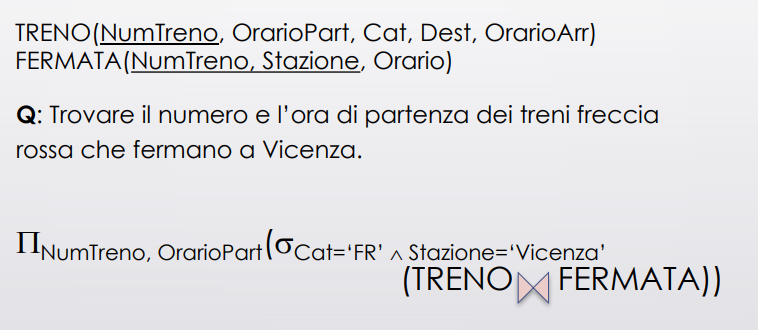
\includegraphics[width=1\linewidth]{image83}
	\caption[]{Esempio di applicazione delle trasformazioni}
	\label{fig:image83}
\end{figure}
\begin{figure}[H]
	\centering
	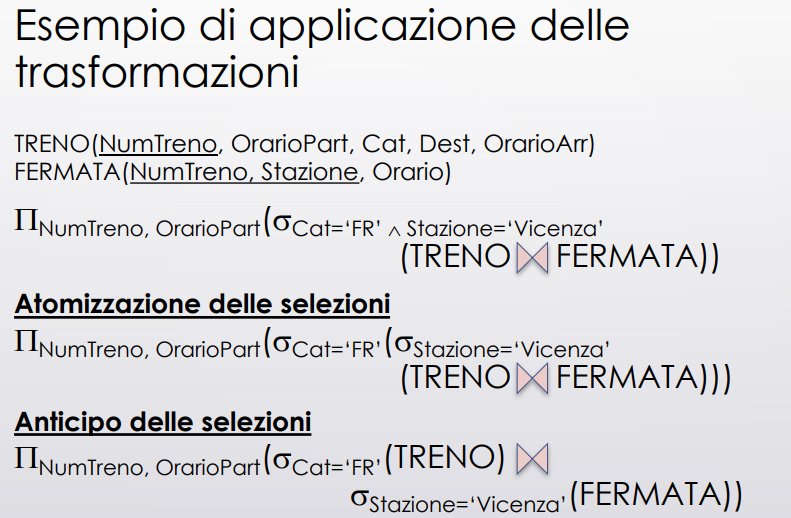
\includegraphics[width=1\linewidth]{image84}
	\caption[]{Esempio di applicazione delle trasformazioni}
	\label{fig:image84}
\end{figure}
\begin{figure}[H]
	\centering
	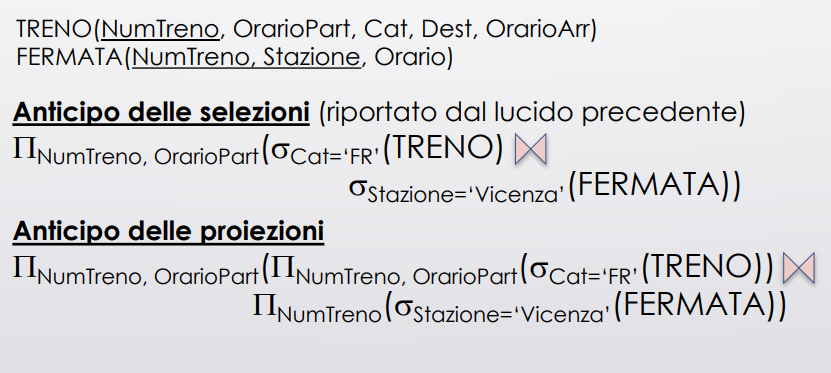
\includegraphics[width=1\linewidth]{image85}
	\caption{Esempio di applicazione delle trasformazioni}
	\label{fig:image85}
\end{figure}
\subsection*{Ulteriori trasformazioni di equivalenza}

Siano $E_1$ ed $E_2$ espressioni di schema rispettivamente $X_1$ e $X_2$.
Si definisce la seguente trasformazione di equivalenza.

\subsubsection*{Inglobamento di una selezione in un prodotto cartesiano}

Questa trasformazione consente di inglobare una selezione applicata a un prodotto
cartesiano in un join con condizione:

\[
\sigma_F(E_1 \times E_2) \;\equiv\; E_1 \bowtie_F E_2
\]

La trasformazione è applicabile solo se:
\[
X_1 \cap X_2 = \emptyset
\]

\noindent
Si osservi che questa regola va applicata solo dopo aver verificato che non sia
possibile anticipare le selezioni rispetto al join.

\begin{figure}[H]
	\centering
	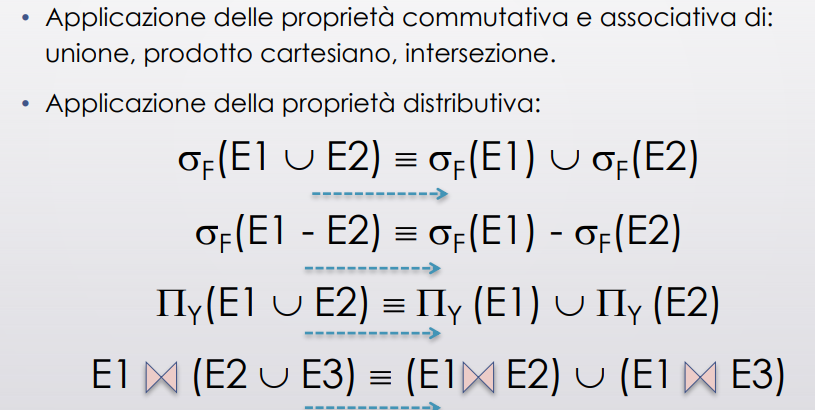
\includegraphics[width=1\linewidth]{image86}
	\caption{Applicazione della proprietà distributiva}
	\label{fig:image86}
\end{figure}
\begin{figure}[H]
	\centering
	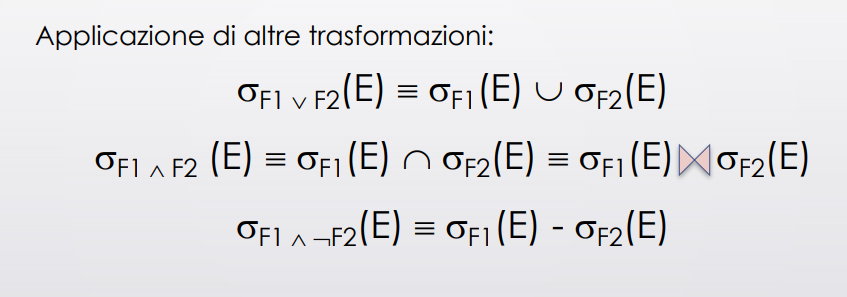
\includegraphics[width=1\linewidth]{image87}
	\caption{applicazione di altre trasformazioni}
	\label{fig:image87}
\end{figure}
\begin{figure}[H]
	\centering
	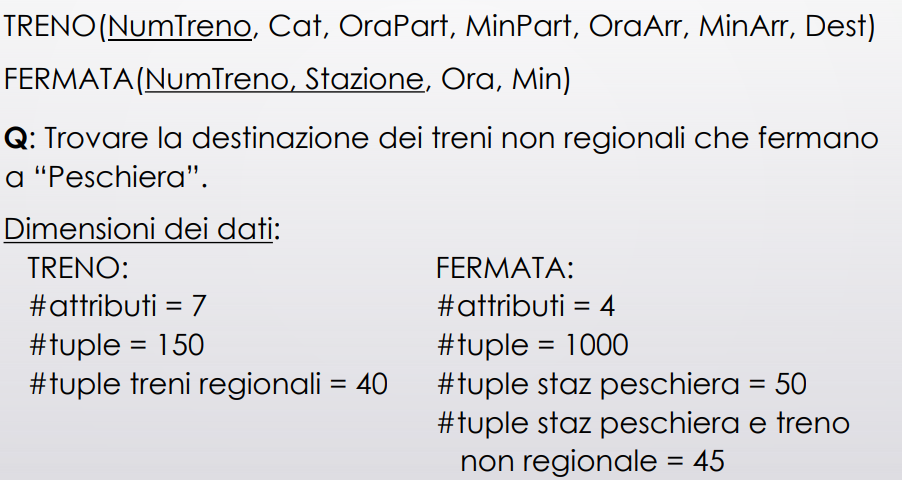
\includegraphics[width=1\linewidth]{image88}
	\caption{Esempio}
	\label{fig:image88}
\end{figure}

